\documentclass[12pt,a4paper]{report}
\usepackage{url}
\usepackage{graphicx}

\newcommand{\optarg}[1]{\textless#1\textgreater}

\begin{document}
\begin{center}
{\LARGE \bfseries LGram} \\[1em]
{\Large \it A cross--platform memory--efficient ngram calculator}
\end{center}

\subsection*{Introduction}
Ngrams are of the up most importance in computational and corpus linguistics. Lgram is a cross--platform tool for calculating ngrams in a memory--efficient manner. The current crop of n-gram tools have non--constant memory usage (see the Comparisons section) such that ngrams cannot be computed for large input texts. Given the prevalence of large texts in computational and corpus linguistics, this deficit is problematic. Lgram has constant memory usage so it can compute ngrams on arbitrarily sized input texts. Lgram achieves constant memory usages by periodically syncing the computed ngrams to an sqlite database stored on disk. The database has support for for around $256^8$ types each of which can occur $256^8$ times. Once all ngrams have been computed the database is used to create a sorted frequency list of ngrams (again with constant memory usage). The database can even be used to compute more exotic ngram forms (such as discontinuous ngrams) although this functionality is not yet provided by lgram.

The lgram processing pipeline proceeds as follows. 
\begin{center}
\begin{minipage}[h]{0.5\textwidth}
\begin{verbatim}
buffers -> blocks -> words -> ngrams
\end{verbatim}
\end{minipage}
\end{center}

A buffer is a chuck of text; blocks are linguistic units as specified by the boundary characters (see the \emph{-b} option). The blocks are split into words and the words are used to compute the ngrams. Special care is taken to make sure ngrams which transverse buffers are computed correctly. The advantage of this method is low memory usage.

\subsection*{Usage}
The functionality of lgram can be customised using command line options. Command--line options come in two equivalent forms; short (\emph{e.g.} \textbf{-n}) and long (\emph{e.g.} \textbf{-{}-ngram}). Only the short form is available on windows. After all options have been specified a list of input files to process has to be provided (see Example section) unless \textbf{-f} is used. All specified input files are processed and stored in the same database.

\subsubsection{-n -{}-ngram \optarg{m--n $\mid$ n}}
This option sets the order of the ngrams to be computed. The order can be specified as either a single number, \emph{i.e.} -n 3 in which case the order is 1-3; or the order can be specified as a range, \emph{i.e.} 2-4. If the order is specified as 4-4 only ngrams of order 4 are computed. The maximum order is 9 and the default order is 1-4. 

\subsubsection{-f -{}-file-list \optarg{filename}}
Instead of reading input files from the command--line, read input files from \emph{filename}. Each line of \emph{filename} should be the name of a single file to process.

\subsubsection{-d -{}-database  \optarg{dbname}} 
Lgram always creates a database when computing ngrams but by default that database is deleted when lgram finishes. Specifying the \textbf{-d} argument saves the database as \emph{dbname}.

\subsubsection{-o -{}-output-file \optarg{filename}}
By default, all ngrams are printed to stdout. Specifying the \textbf{-o} options also saves the ngrams to \emph{filename}.

\subsubsection{-O -{}-output-by-n \optarg{filename}} 
Rather than saving the ngrams to a single file, option $\textbf{-O}$ saves the ngrams to multiple files named \emph{filename-k} where $k$ is the order of the ngram (see Example section).

\subsubsection{-r -{}-regex--file \optarg{filename}}
Apply each regex in \emph{filename} to each block processed by lgrams. The regex file must be in the following format.
\begin{verbatim}
regex1   <tab>   replace_string1
# comment
regex2   <tab>   replace_string2
\end{verbatim}
such that the regular expression and the replacement string are tab separated. The regex is a global replace and the regex format is PCRE (Perl compatible). If there is no replace string the regex matches are replaced with nothing (\emph{i.e.} they are removed). For instance if the user wishes to remove all double quotes the following regex would suffice:
\begin{verbatim}
"\s*
\end{verbatim}
without the \texttt{\textbackslash s*} part, whatever succeeds the double quote may be ngram'ed with a space character.

\subsubsection{-b -{}-boundary \optarg{str}}
Ngrams are not calculated across boundary characters. The default string is \emph{.,?!:;} so that ngrams are not calculated across sentences or divisions of sentences.

\subsubsection{-B -{}-ignore-boundary}
By default the boundary characters are treated as tokens and included in ngrams, if \textbf{-B} is enabled ngrams which contain boundary characters are ignored.

\subsubsection{-u -{}-preserve-case}
By default all letters are transformed to lower case, \textbf{-u} prevents this behaviour.

\subsubsection{-s -{}-no-stdout}
Do not print ngrams to stdout. This options should be used in conjunction with \textbf{-o}, \textbf{-O} and \textbf{-d}.

\subsubsection{-q -{}-quiet}
Don't print anything but errors

\subsection*{Example}
Let us compute 1-grams to 4-grams on Bram Stokers Dracular\footnote{\url{http://www.gutenberg.org/ebooks/345}}
\begin{verbatim}
lgram -n 4 -s -O BSD-ngram -d BSD.db bs-dracular.txt
\end{verbatim}
Running this commands gives the output:
\begin{verbatim}
[1] bs-dracular.txt [29s]
[+] building 1gram frequency list
[+] building 2gram frequency list
[+] building 3gram frequency list
[+] building 4gram frequency list

processed 445537 ngrams in 41s
\end{verbatim}
and the five files:
\begin{verbatim}
BSD.db
BSD-ngram-1
BSD-ngram-2
BSD-ngram-3
BSD-ngram-4
\end{verbatim}
\texttt{BSD.db} is the sqlite database. If the \textbf{-d} argument was not specified, the database would have been deleted after the ngrams were saved. The \texttt{BSD-ngram} files contain sorted lists of ngrams and their frequency. For instance, the first 5 lines of \texttt{BSD-ngram-3} are:
\begin{verbatim}
i could see 71
i could not 65
there was a 63
i did not 56
a sort of 49
\end{verbatim}

\subsection*{Comparisons}
For a comparisons we choose two widely used ngram tools; NSP\footnote{\url{http://www.d.umn.edu/~tpederse/nsp.html}} and kfNgram\footnote{\url{http://www.kwicfinder.com/kfNgram/kfNgramHelp.html}}. All tests were performed on a 2Ghz desktop computer, all settings were made as equivalent as possible. These values are for computing 4-grams across a range of literature.

\begin{center}
\begin{minipage}[h]{0.4\textwidth}
\centering
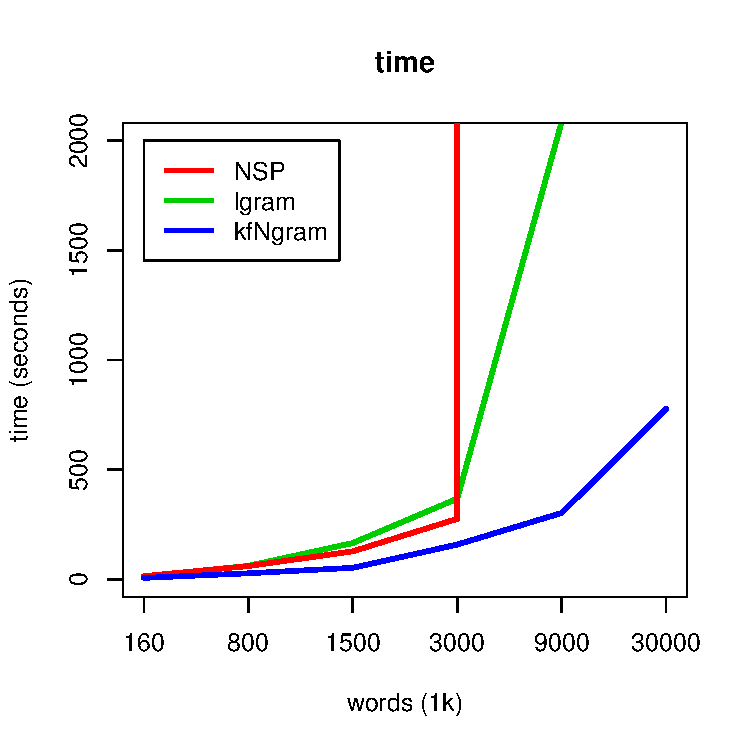
\includegraphics[scale=0.55]{time.pdf}
\end{minipage}
\hspace{3em}
\begin{minipage}[h]{0.4\textwidth}
\centering
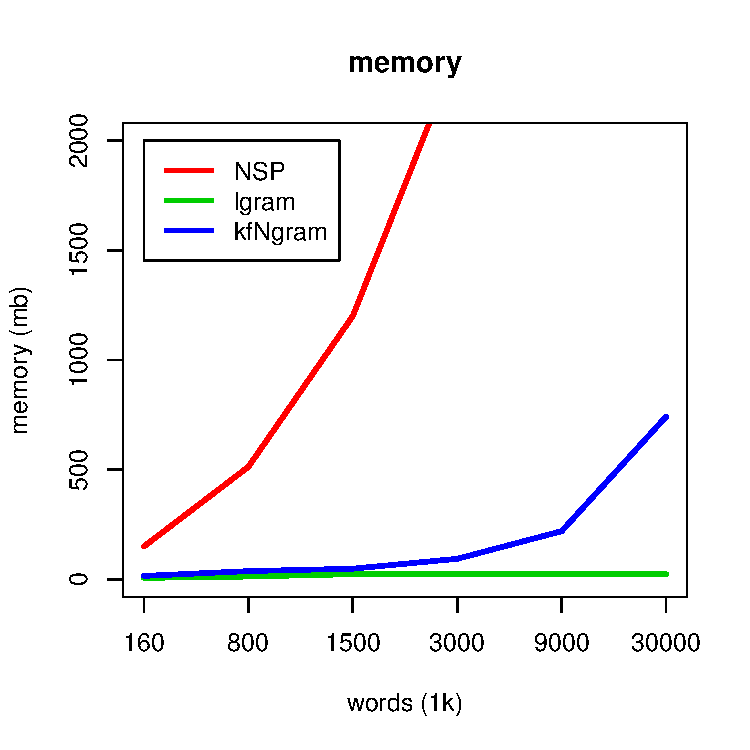
\includegraphics[scale=0.55]{memory.pdf}
\end{minipage}
\end{center}

We see that lgram has constant memory usage but is slower as a result. It takes around 7 hours to compute 4-grams on 30 million words. NSP is fast but cannot calculate ngrams on texts above 3 million words on a computer with 4gb of ram. KfNgram performs best although it does not have constant memory usage and it cannot be run in Unix. In the future we would like to incorporate features of KfNgram to speed up lgram.

\subsection*{Requirements}
Lgram requires libpcre/libpcrecpp for regular expressions and libsqlite3 for the database. For windows the libraries are included in the precompiled executable of lgram but you must install the Microsoft Visual C++ 2010 Redistributable Package\footnote{\url{http://www.microsoft.com/download/en/details.aspx?id=14632}}. For Unix and Mac the libraries can be installed using your package manager or download from \url{pcre.org} and \url{sqlite.org}.

\subsection*{Credits}
Lgram was written by Edward J. L. Bell\footnote{\url{ejlbell@gmail.com}} at Lancaster University\footnote{\url{http://www.lancs.ac.uk}} and funded by UCREL\footnote{\url{http://ucrel.lancs.ac.uk}}. The project was initiated by Dr Paul Rayson\footnote{\url{http://www.comp.lancs.ac.uk/~paul}}. Lgram is open--source and released under the GPL license.

\end{document}
